 %美赛模板:正文部分

\documentclass[12pt]{article}  % 官方要求字号不小于 12 号,此处选择 12 号字体
% \linespread{1.1}
% \bibliographystyle{plain}
% 本模板不需要填写年份,以当前电脑时间自动生成
% 请在以下的方括号中填写队伍控制号
\usepackage[2409015]{easymcm}  % 载入 EasyMCM 模板文件
\problem{C}  % 请在此处填写题号
% \usepackage{mathptmx}  % 这是 Times 字体,中规中矩 
\usepackage{palatino}  % mathpazo 这palatino是 COMAP 官方杂志采用的更好看的 Palatino 字体,可替代以上的 mathptmx 宏包
\usepackage{pdfpages}
\usepackage{longtable}
\usepackage{tabu}
\usepackage{threeparttable}
\usepackage{listings}
\usepackage{paralist}
\usepackage{makecell}
\usepackage{geometry}
\usepackage{booktabs}
\usepackage{tabularx}
\usepackage{graphicx}
\geometry{letterpaper, margin=1in}

\graphicspath{{img/}}          % 此处{img/}为相对路径,注意加上“/”
 \let\itemize\compactitem
 \let\enditemize\endcompactitem

\newcommand{\upcite}[1]{\textsuperscript{\textsuperscript{\cite{#1}}}}
\title{M}  % 标题

% 如需要修改题头(默认为 MCM/ICM),请使用以下命令(此处修改为 MCM)
%\renewcommand{\contest}{MCM}

 %文档开始
\begin{document}

% 此处填写摘要内容
\begin{abstract}
    
 to the e s Engineering

    % 美赛论文中无需注明关键字。若您一定要使用,
    % 请将以下两行的注释号 '%' 去除,以使其生效
    \vspace{5pt}  %mm	毫米	1 mm = 2.845 pt   pt 点	1 pt = 0.351 mm
    \textbf{Keywords}:ARIMA; Fish Migration; Earnings Evaluation; Computer Simulation

\end{abstract}

\maketitle  % 生成 Summary Sheet

\tableofcontents  % 生成目录


% 正文开始
% Chapter 1: Introduction
\section{Introduction}

\subsection{Problem Background}
In today's society, tennis has evolved into one of the most visually appealing and fan-favorite sports globally. 
As of 2022, the sport has reached an impressive milestone in terms of global participation. 
There are over 100 million tennis players worldwide, encompassing all levels from amateur to professional, 
a figure that has been steadily increasing over the past decade.
Moreover, the long history of tennis is marked by many memorable matches due to their uniqueness, intensity, 
or historical significance. For instance, the 2023 Wimbledon men's singles final was a case in point. 
In this match, 20-year-old Spanish rising star Carlos Alcaraz triumphed over 36-year-old Novak Djokovic, 
thereby ending the spectacular record of one of the greatest Grand Slam players in history. 
This match was characterized by its dramatic twists and turns and continuous excitement. 
Both players experienced incredible fluctuations in performance, at times dominating the play and at others being dominated. 
This phenomenon may relate to the concept of 'momentum' experienced by a team or player in a sport. In this report, 
our team aims to use scientific and mathematical methods to measure and predict this seemingly intangible concept in the context of the match.


\subsection{Restatement of the Problem}
In this study, our team obtained data for every point played in the men's singles matches at Wimbledon 2023, 
starting from the third round onwards. 
This data acquisition was aimed at addressing the following questions:
\begin{itemize}
\setlength{\parsep}{0ex} %段落间距
\setlength{\topsep}{2ex} %列表到上下文的垂直距离
\setlength{\itemsep}{1ex} %条目间距
\item Create a model leveraging existing datasets to analyze and identify the dominating player or team at certain points in a match. 
This model should quantify their advantage and include a visualization feature. 
Moreover, the model should be customized for various sports. 
For instance, in tennis matches, 
it should reflect the server's higher likelihood of scoring. 
This approach will showcase the model's adaptability across different sports.
\item Employ the developed model to evaluate a coach's viewpoint by analyzing if the fluctuations 
in a player's 'momentum' during a match are due to random changes.
\item Based on existing data, create a new model to predict fluctuations in player performance 
during a match and identify the indicators most closely related to shifts in the game's dynamics. 
Simultaneously, use the data on past fluctuations in players' 'momentum' to provide strategies for upcoming matches between two players.
\item Conduct trials of the model across different matches and sports to assess its effectiveness in prediction and 
its applicability to sports beyond tennis. 
Following these trials, identify the model's limitations and propose additional factors that might influence its performance.
\item Compile the insights from your experiments to offer guidance about 'momentum' to tennis coaches and players. 
This will aid them in developing strategies for handling situations that affect the course of tennis matches.
\end{itemize}


\subsection{Our Work}
In athletic competitions, 'momentum' typically signifies the cumulative 'force' or 'drive' generated from various events. 
Although it's an intangible concept and challenging to measure, this task involves investigating how to quantify momentum using match data. 
We'll examine the impact of different events on momentum shifts and, using our results, 
offer targeted strategies for tennis coaches and players. Our key responsibilities include:
\begin{enumerate}[\bfseries 1.]
    \setlength{\parsep}{0ex} %段落间距
    \setlength{\topsep}{0.5pt} %列表到上下文的垂直距离
    \setlength{\itemsep}{0.5pt} %条目间距
    \item By harnessing point-by-point data from the 2023 Wimbledon men's singles (beyond the initial two rounds) and integrating it 
    with publicly accessible match statistics online, we aim to gather detailed player profiles and match data. 
    This approach will facilitate a more precise quantification and examination of momentum.
    \item Based on the existing data, develop a model that can quantitatively determine which player or team has the advantage at specific times 
    during a match. Visualize this model to assess the randomness of fluctuations throughout the course of the game.
    \item Develop a forecast model aimed at predicting variations in players' performances throughout a match, 
    pinpointing key elements that are significantly related to pivotal moments in the match.
    \item Gather and systematize match data across diverse events and sports types to evaluate 
    the predictive accuracy of the model and its applicability beyond tennis. Additionally, 
    enhance the model by including elements that were initially overlooked.
    \item Based on the model's results, provide specific advice and strategies for coaches and players in the sport of tennis.
\end{enumerate}

\section{General Assumptions}
Considering that practical problems always contain many complex factors, first of all, we need to make reasonable assumptions to simplify the model, and each hypothesis is closely followed by its corresponding explanation:

\begin{enumerate}[\bfseries \textit{Assumption} 1:]
	\item \textbf{At the beginning of a tennis match, the 'momentum' for each player or team is equally established at a value of 0.}\\
	\textbf{\textit{Explanation:}}In tennis matches, it's important to note that under certain circumstances, 
    there can be a significant difference in 'momentum' between the players before the match even begins. 
    An example is a match between someone completely unfamiliar with tennis and a world champion, 
    where their 'momentum' could differ significantly before the start. However, to simplify the model, 
    reduce the difficulty of data collection and processing, 
    our team has decided that 'momentum' in the match will only be related to the players' behavior during the game and not influenced 
    by external factors. 
    Therefore, we have set the initial 'momentum' values for both sides to be the same.
	\item \textbf{In tennis, matches played repeatedly between the same pair of players are treated as separate and independent events with no influence on each other.}\\
	\textbf{\textit{Explanation:}}The second hypothesis builds upon the first. 
    For model simplification and to ease the data collection and processing efforts, 
    our team's analysis is concentrated on the shifts in 'momentum' within the confines of 'sets', 'games', and 'points' 
    during a single tennis match. Consequently, it's established that the initial 'momentum' for both players is identical and does not vary, 
    irrespective of the number of times they have competed against each other.
	\item \textbf{The variations in 'momentum' for a particular player during a tennis match are predictable.}\\
	\textbf{\textit{Explanation:}}While a player's momentum in tennis is linked to both competitors' actions, 
    individual factors like habits, physical condition, 
    and preferences mean that a particular player's skill and tactical approach tend to remain stable across various matches. 
    Consequently, our team can use historical data on a specific player's 'momentum' fluctuations to forecast future game data changes, 
    enabling us to offer tailored recommendations before upcoming matches.
\end{enumerate}



\section{Notations}
Some important mathematical notations used in this paper are listed in Table 1. 
\begin{table}[htbp]
\begin{center}
\caption{Notations used in this paper}
\begin{tabular}{c l}
\toprule[2pt]
\multicolumn{1}{m{3cm}}{\centering Symbol}
&\multicolumn{1}{m{8cm}}{\centering Description }\\
\midrule
$x$& Longitude \\
$y$& latitude \\
$t$& The time from now \\
$u(x,y,t)$& The temperature after t years at the location with Coordinates(x, y)\\
$v(x,y,t)$& The speed after t years at the location with Coordinates(x, y) \\
$C(t)$ & The cost for fishing t years later \\
$P(t)$ & The income for fishing t years later \\
$I(t)$ & The profit for fishing t years later \\
\bottomrule[2pt]
\end{tabular}\label{tb:notation}
 \begin{tablenotes}
        \footnotesize
        \item[*] *There are some variables that are not listed here and will be discussed in detail in each section. %此处加入注释*信息
      \end{tablenotes}
\end{center}
\end{table}
\vspace{-1cm}%在\end{table}下加一行\vspace{-1cm} 其中-1的作用是缩短与下方文字距离的 切记!必须是负数


\section{Data}
\subsection{Data Collection}
For this project, we have already obtained data for every point after the first two rounds of the 2023 Wimbledon men's singles. 
However, to test the generalizability of our team's model as required by the task, 
we have still sourced some publicly available match data on the internet, which includes:

\begin{table}[htbp]
\begin{center}
\caption{Data and Database Websites}
\resizebox{\textwidth}{!}
{\begin{tabular}{c c}
\toprule[2pt]
\multicolumn{1}{m{5cm}}{\centering \textbf{Database Names}}
&\multicolumn{1}{m{10cm}}{\centering \textbf{Database Websites} }\\ %m后面是列宽
\midrule
APDRC & http://apdrc.soest.hawaii.edu/ \\
NOAA & https://www.noaa.gov/ \\
HadISST & https://www.kaggle.com/carlosparadis/ \\ 
\bottomrule[2pt]
\end{tabular}}
\end{center}
\end{table}

\subsection{Data Processing}
In the data cleansing phase, our team executed various cleaning operations. For instance, 
in the dataset of every point post the first two rounds of the 2023 Wimbledon men's singles, 
we found missing entries in Serve speed, serve direction, serve depth and return depth, 
amounting to 752, 54, 54, and 1309 values respectively. We compensated for these gaps by averaging and judiciously removing data, 
and also eliminated outliers in parameters such as movement distance and stroke count using both mathematical methods and manual review. 
This cleaning procedure was similarly applied to additional datasets sourced from the web.

\section{Model Preparation I}
According to the task requirements, our team, using the available data, 
has developed a model that can quantitatively determine which player or team is more dominant at specific times in a match. 
Clearly, this 'dominance' is what we refer to as the player's 'momentum', an abstract concept influenced by multiple factors. 
Facing this seemingly intangible concept in matches, 
our team's most crucial goal is to quantify it. With this objective in mind, we initiated the next phase of our work.

\subsection{Engineering of Features}
It's evident that we're dealing with a 'big data' challenge here. 
Our team dedicated a lot of time and effort to data analysis and processing in hopes of deriving valid indicators. 
A pivotal part of this task and the foundation of our model — quantifying 'momentum' — led us to extensively review scholarly 
articles and literature. 
However, we discovered that in tennis, there isn't a standardized definition or quantifiable measure for a player's 'momentum'. 
The dictionary defines 'momentum' as 'force accumulated through movement or a sequence of events', and in the realm of sports, 
coaches and athletes typically use 'momentum' to denote a kind of advantage during a match.

Based on previous discussions and data we researched online, 
our team concludes that in tennis, 'momentum' for players is shaped by short-term aspects like specific technical moves 
(for example, the server scoring, as mentioned in the task) and long-term elements such as a series of successful points. 
These factors collectively manifest as a player's dominance over the flow of the match, signifying their advantage. 
It naturally follows that a player with this advantage has a higher chance of winning the rally, 
and there's a strong correlation between the two. Therefore, we infer that elements significantly impacting a player's chance of winning 
might also heavily influence their 'momentum'. 
Our team aims to uncover these influential factors to serve as metrics for evaluating and quantifying a player's 'momentum'.

Based on the 2023 Wimbledon men's singles data provided in the task, 
our team used the win rate that can be directly calculated from the dataset to identify the features 
that most positively impact player win rates. First, we calculated the win rate for each player on a 'point' basis within a match. 
To comprehensively evaluate players' win rates, we extracted corresponding data for each player from the available dataset, 
such as the number of serves, break points, and net approaches, and constructed a correlation matrix:
\begin{figure}[htbp]  %h此处,t页顶,b页底,p独立一页,浮动体出现的位置
    \centering  %图表居中
    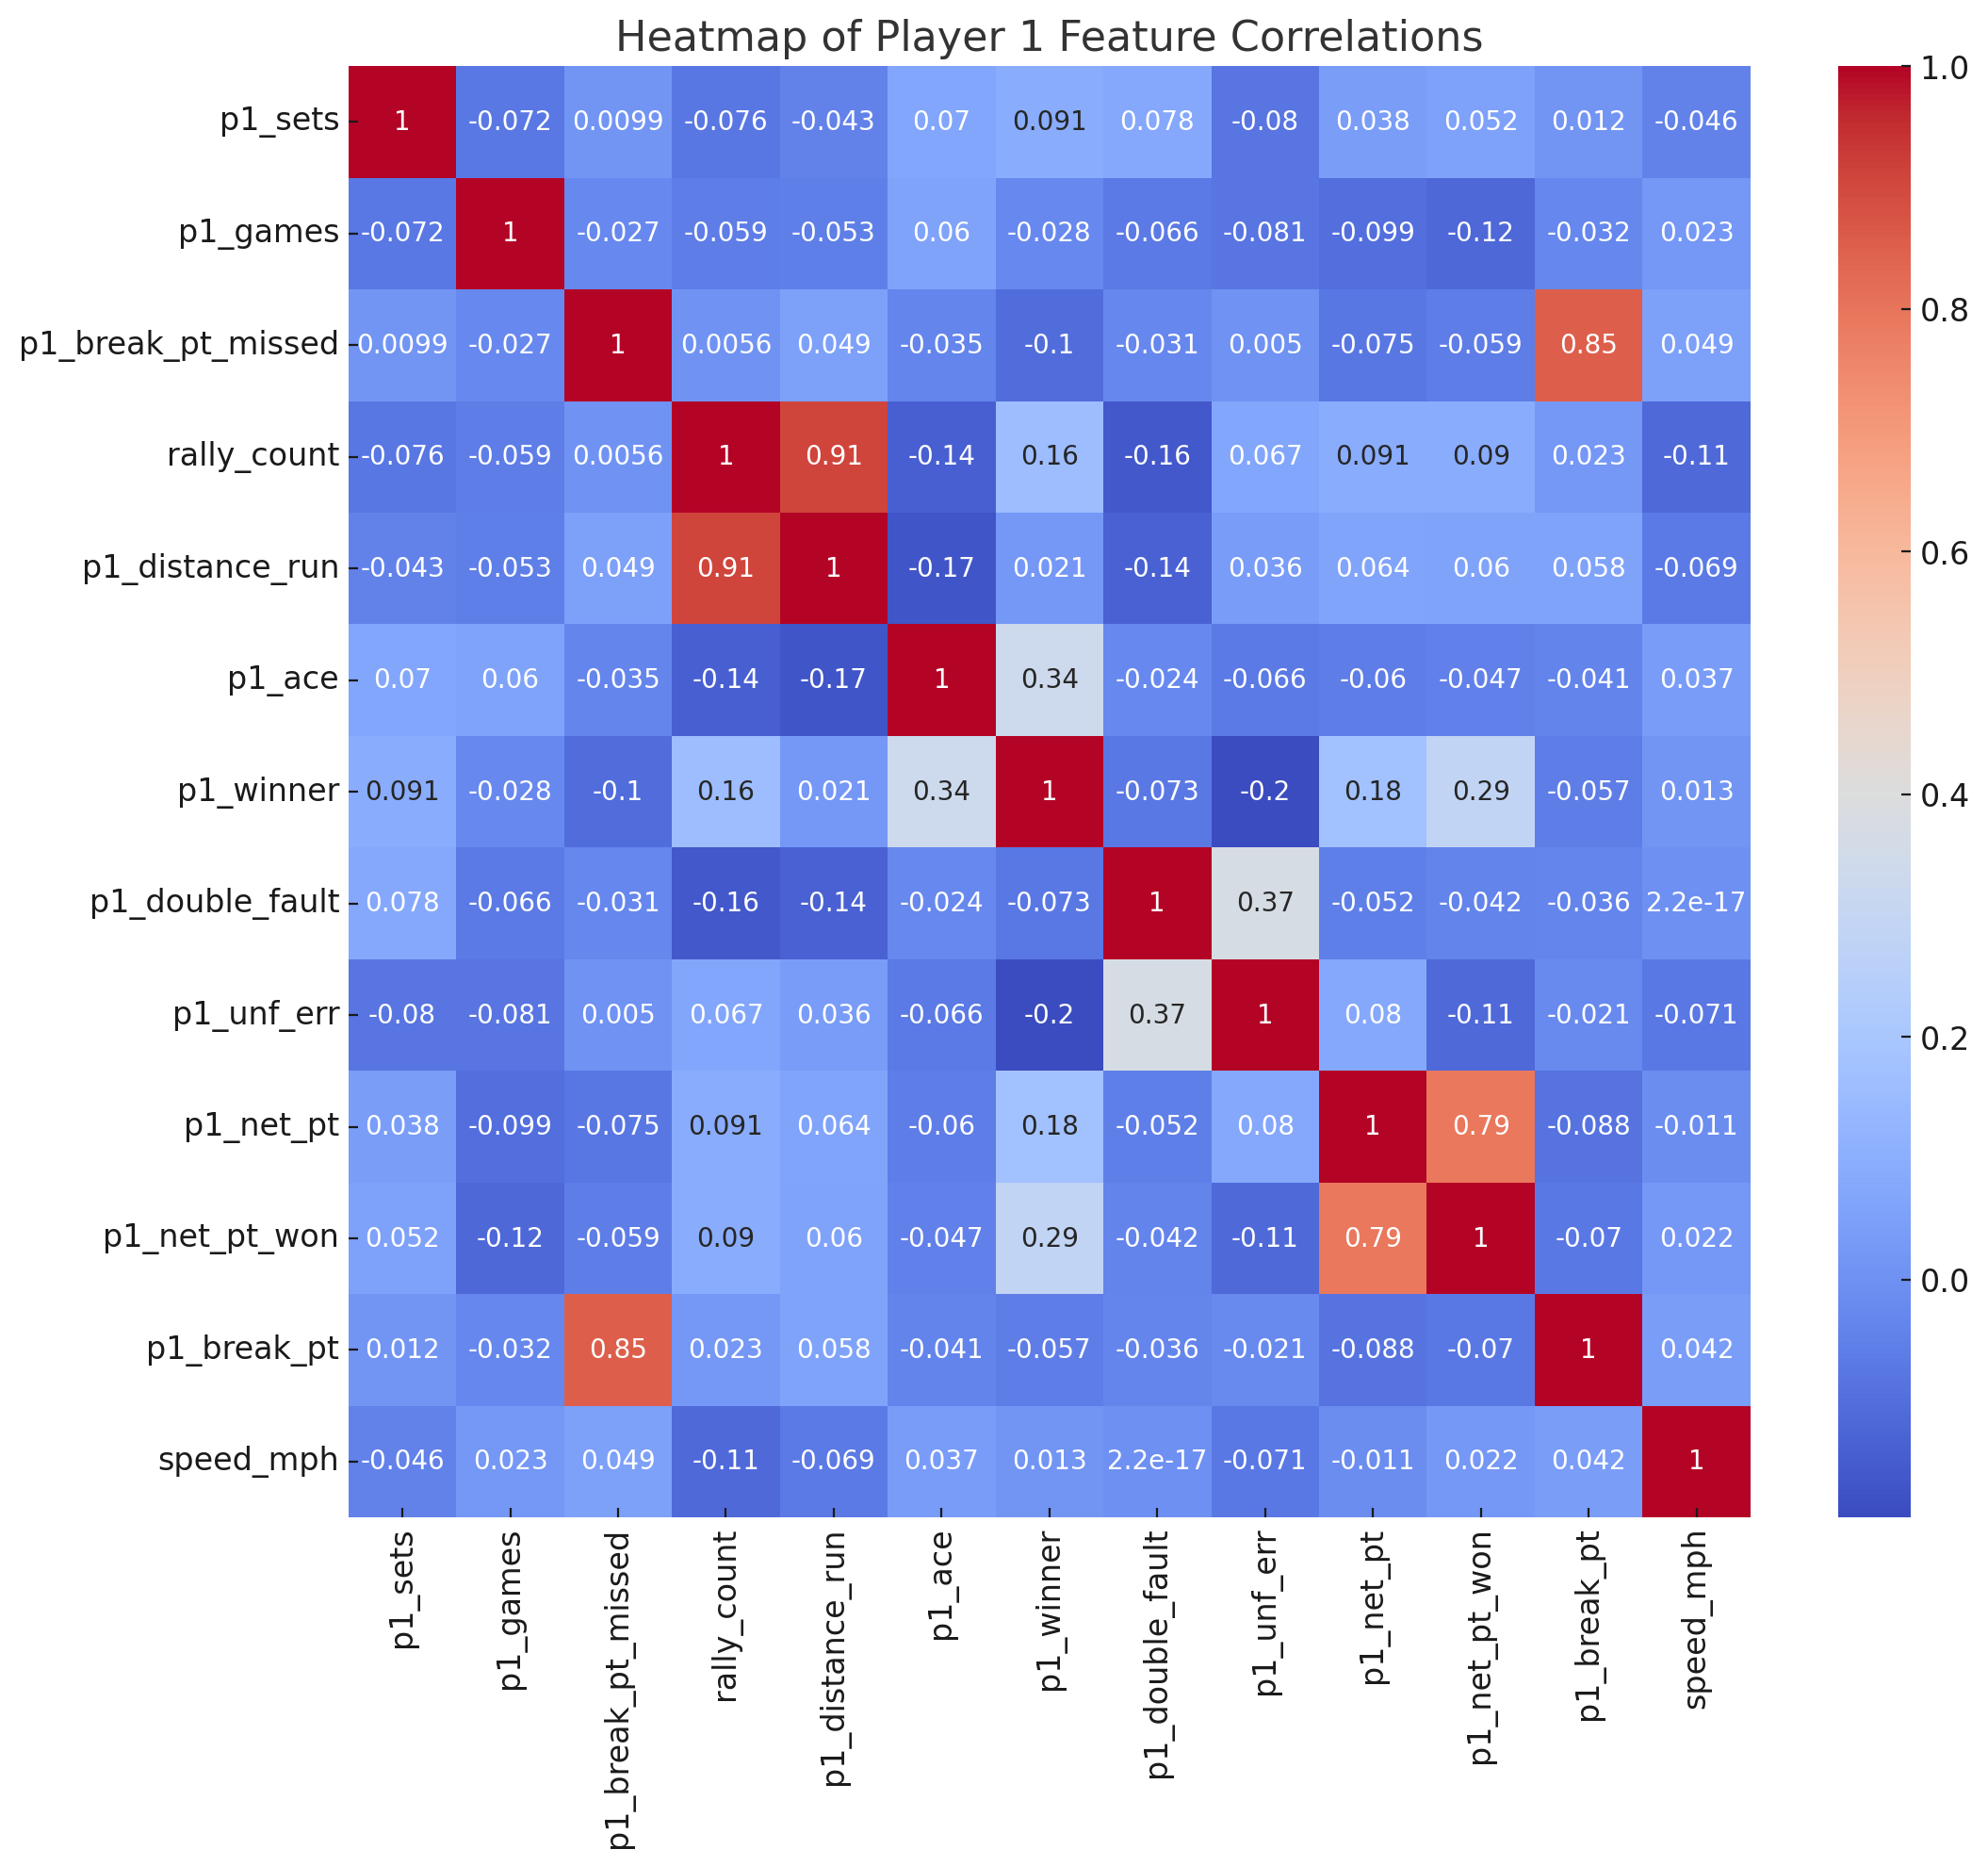
\includegraphics[width=.6\textwidth]{1.png} %图片的名称或者路径之中有空格会出问题 
    \caption{Correlation matrix} % 图片标题 
\end{figure}

Based on the correlation matrix, we noted significant correlations among certain features 
and the presence of numerous variables in the dataset. 
This necessitates the application of dimensionality reduction techniques to these variables:
\begin{figure}[htbp]  %h此处,t页顶,b页底,p独立一页,浮动体出现的位置
    \centering  %图表居中
    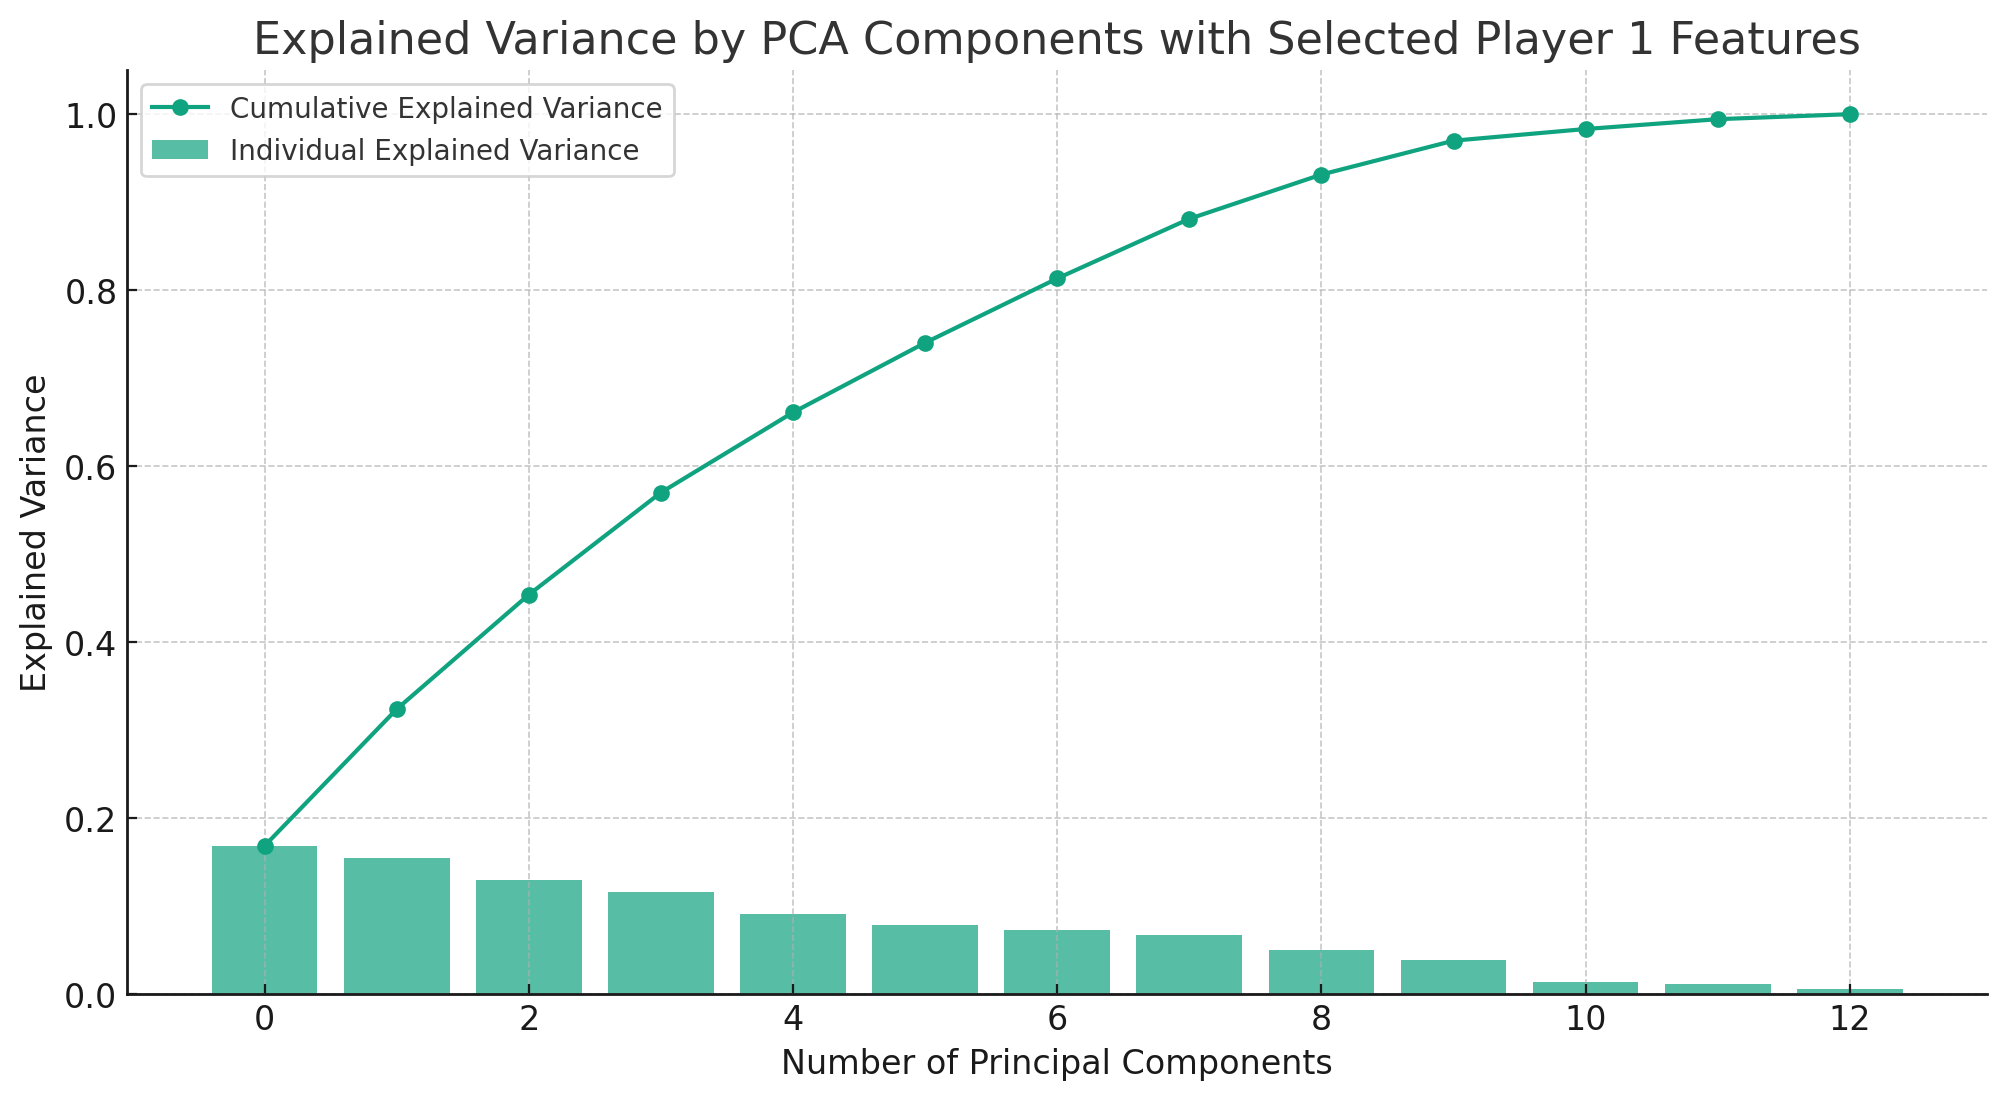
\includegraphics[width=.7\textwidth]{2.png} %图片的名称或者路径之中有空格会出问题 
    \caption{PCA} % 图片标题 
\end{figure}

As indicated in the previous graph, the cumulative contribution of the first nine principal components accounts for 90\% of the variance. 
For the sake of simplifying our analysis, we will omit the components beyond the ninth. 
Next, we assess the correlation between these nine principal components and the players' winning probabilities, 
as depicted in the subsequent graph:
\begin{figure}[htbp]  %h此处,t页顶,b页底,p独立一页,浮动体出现的位置
    \centering  %图表居中
    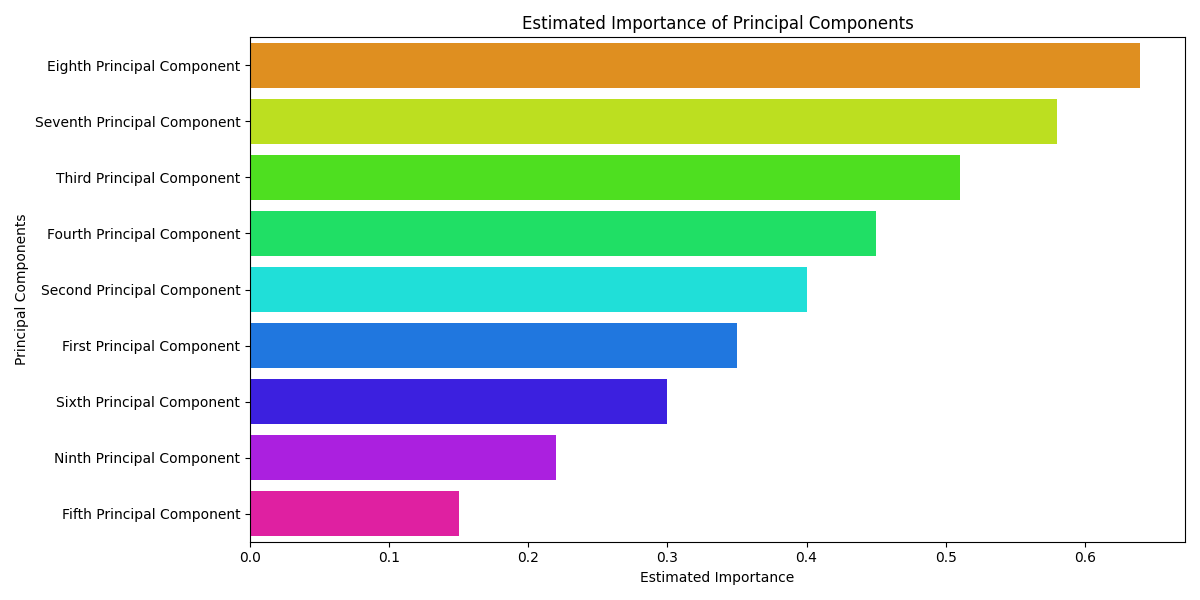
\includegraphics[width=.7\textwidth]{3.png} %图片的名称或者路径之中有空格会出问题 
    \caption{Estimated Importance of Principal components} % 图片标题 
\end{figure}

The first six principal components depicted in the graph are arguably the most significant factors affecting players' 
win rates within our dataset. By examining the linear associations between these six principal components and the initial features,
 we can pinpoint the most relevant features to these principal components. 
These key features will act as the primary metrics for evaluating 'momentum' in our model.

Additionally, our feature extraction endeavor extends beyond the initial steps. 
We explored various scholarly articles and publications available online that might relate to our study. 
In this exploration, we discovered several technical metrics, such as the success rate of first serves, 
scoring on return against the first serve, serving speed, scoring rate on first serves, effectiveness in saving break points, 
success rate at the net, and scoring percentage from the baseline. These indicators were extracted and processed from the existing data, 
undergoing evaluations similar to the aforementioned processes. 
Due to the complexity of these procedures, I won't delve into the details here.

As a result, our team, informed by the existing data, relevant scholarly work, 
and our collective insight into players' 'momentum' during tennis matches, 
has identified the following key evaluation metrics:


\subsection{Model Construction}
Evidently, in the context of this project, 
the pivotal aspect of our model lies in quantifying the 'momentum' of a player. From our feature extraction efforts, 
we've pinpointed several elements that impact a player's 'momentum'. Thus, our team adopted a fundamental and direct approach to assessment.
 We perceive a player's 'momentum' as their on-court advantage. A player should earn 'momentum' points 
 for performing advantageous technical actions or achieving a series of scores that elevate their spirit, 
and conversely lose points otherwise. The basic premise of our team's model can be encapsulated in the subsequent formula:
\begin{align} % 公式环境
    M_t = \alpha X_t - \beta Y_t
\end{align}
In this formula, $M_t$ represents the comprehensive momentum score, 
$X_t$ indicates the positive contribution to momentum by a player's actions at time point 't', 
and $Y_t$ represents the negative contribution to momentum by a player's actions at time point 't'. 
$ \alpha $ and $ \beta $ are weight parameters that need to be obtained through training.

Based on the indicators previously selected by our team, 
we have also specified scoring for each type of action. 
Firstly, there's the basic scoring part: if a player wins a 'point' in a 'game' during the match, 
their 'momentum' score increases by one, and conversely, there's a corresponding deduction for losing a point. 
Secondly, considering that a player might score consecutively or even win several 'games' or 'sets' in a row, 
we took into account the impact of consecutive scoring and winning streaks on momentum. 
Our team also considered how the margin of victory during a winning streak affects momentum. 
For the scoring of consecutive points and game victories, we adopted a linear adjustment method. 
In terms of the impact of the score difference on player momentum, 
our team conducted numerous trials and manual adjustments. 
We ultimately concluded that the impact of score differences in 'sets' and 'games' on player momentum is distinct. Clearly, in matches, 
the difference in the number of sets won has a greater impact on a player's performance. Therefore, our team has chosen the following formula:
\begin{align} % 公式环境
    S_t = \alpha * S_n + \beta * 2^{S_n}\\
    G_t = \alpha * G_n \\
    P_t = \alpha * P_n
\end{align}
In this formula,$S_t$ ,$G_t$  and $P_t$ signifie the score corrections at time 't' for a player 
on a winning streak for their consecutive victories in 'sets', 'games', and 'points'. 
$S_n$ ,$G_n$  and $P_n$ indicate the counts of consecutive sets, games, and points won by the player at time 't'. As before, 
$ \alpha $,$ \beta $ and $\gamma$ are the weighting parameters, which require calibration through model training.

Based on our feature extraction work, we have thoroughly considered the physical aspect of players during the match. 
Our team combined the number of strokes exchanged between players and the distance they ran, resulting in the following formula:
\begin{align} % 公式环境
    D_t = \alpha R_n + \beta D_n
\end{align}

\subsection{Results}

\section{Volatility stochastic assessment}














\section{Model Preparation II}

\subsection{Model Construction}
In our initial inquiries, we developed a momentum score framework predicated on specific metrics observed during gameplay, 
enabling the computation of each competitor's momentum at the conclusion of every round within a given match.
The objective of discerning the match's pivotal juncture, the round where the dynamics notably shift, 
necessitates an understanding of the on-court realities and the strategies employed by both the offensive and defensive 
players that contribute to this shift. This logically extends from our primary question, directing our attention to the 
intersection of the two momentum trajectories. Yet, this approach surfaces two pertinent challenges:

\begin{enumerate}
    \item The foundational model, as established in our primary query, 
    is anchored in assumptions that are straightforward and intuitively resonant. For the third query, 
    where the focus is on pinpointing match turning points, our predictive model must integrate a broader
    array of features pertinent to serving and returning dynamics 
    (such as 'p1\_ace', 'p2\_ace', 'p1\_double\_fault', 'p2\_double\_fault', 'serve\_width\_B', and others).
    This necessitates employing machine learning techniques to assimilate these feature weights effectively into the momentum curve modeling.

    \item Our initial model presupposes that momentum scores are contingent
     on recent round performances, interpreting 'momentum' as an expression
      of a player's arousal state. Given the fluctuating fortunes in elite 
      tennis matches, momentum shifts are expected to be frequent. This results
       in an overabundance of intersection points on the momentum curves. 
       To address this, it becomes imperative to develop methodologies that 
       filter out insignificant, repetitive stalemate points, thereby 
       concentrating on rounds that signify a transition into or out of a deadlock.
\end{enumerate}

For the first issue, we employed a random forest regressor to train 
our model using data processed through the momentum score model 
established in the first question. The momentum score serves as a 
crucial label in the supervised learning process. We used the $R^{2}$
score as the evaluation metric and observed the importance of features
 post-training. To prevent model overfitting and enhance the 
 generalizability of our predictive model, it's essential to select
  primary features for further training.

Regarding the second issue, we first identify all intersection 
points where the change in momentum is not less than a certain threshold. 
Then, we select those points that do not have any other intersection
points in their vicinity, meaning there are no further momentum 
crosses in several rounds before or after these points. We locate
these turning points and, in conjunction with the specific on-court
situations, analyze the rationality of our predictions.


\subsection{Results}
The figure\ref{feature} shows the ranking of feature importance 
after the initial training.
\begin{figure}[h]  %h此处,t页顶,b页底,p独立一页,浮动体出现的位置
    \centering  %图表居中
    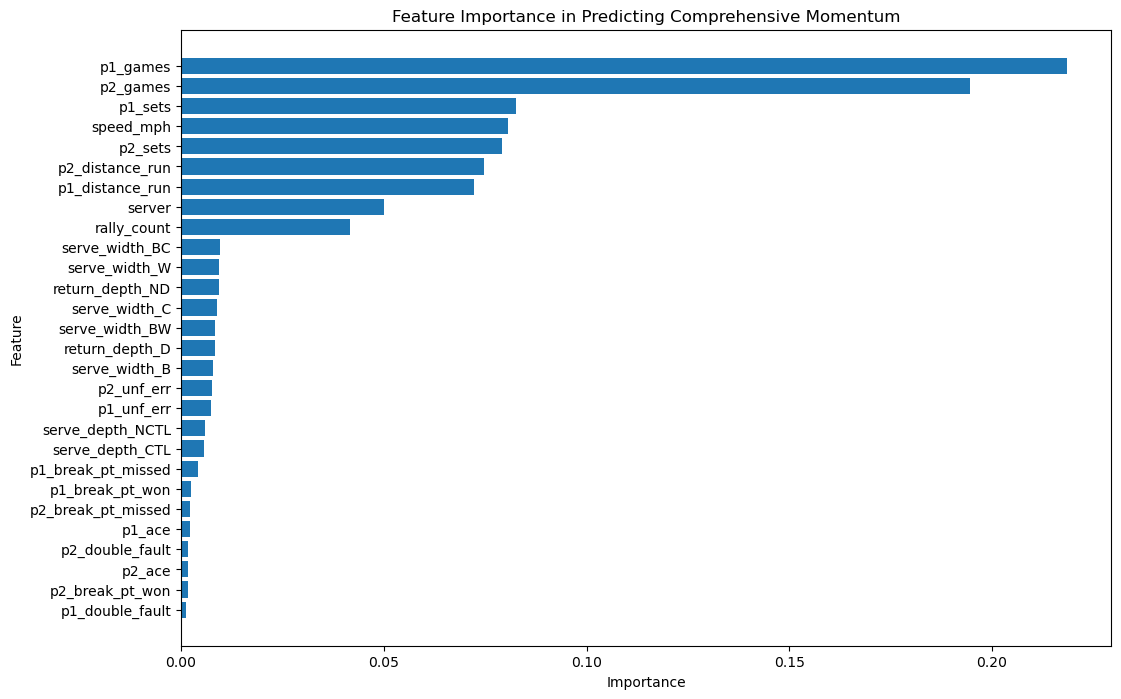
\includegraphics[width=.9\textwidth]{feature_inmportance.png} %图片的名称或者路径之中有空格会出问题 
    \caption{Feature Inportance} % 图片标题 
    \label{feature}
\end{figure}

Select the top 10 features with the highest importance for retraining. 
Then, obtain the actual and fitted momentum curves\ref*{pred_act} for Player1 and Player2.
\begin{figure}[h]  %h此处,t页顶,b页底,p独立一页,浮动体出现的位置
    \centering  %图表居中
    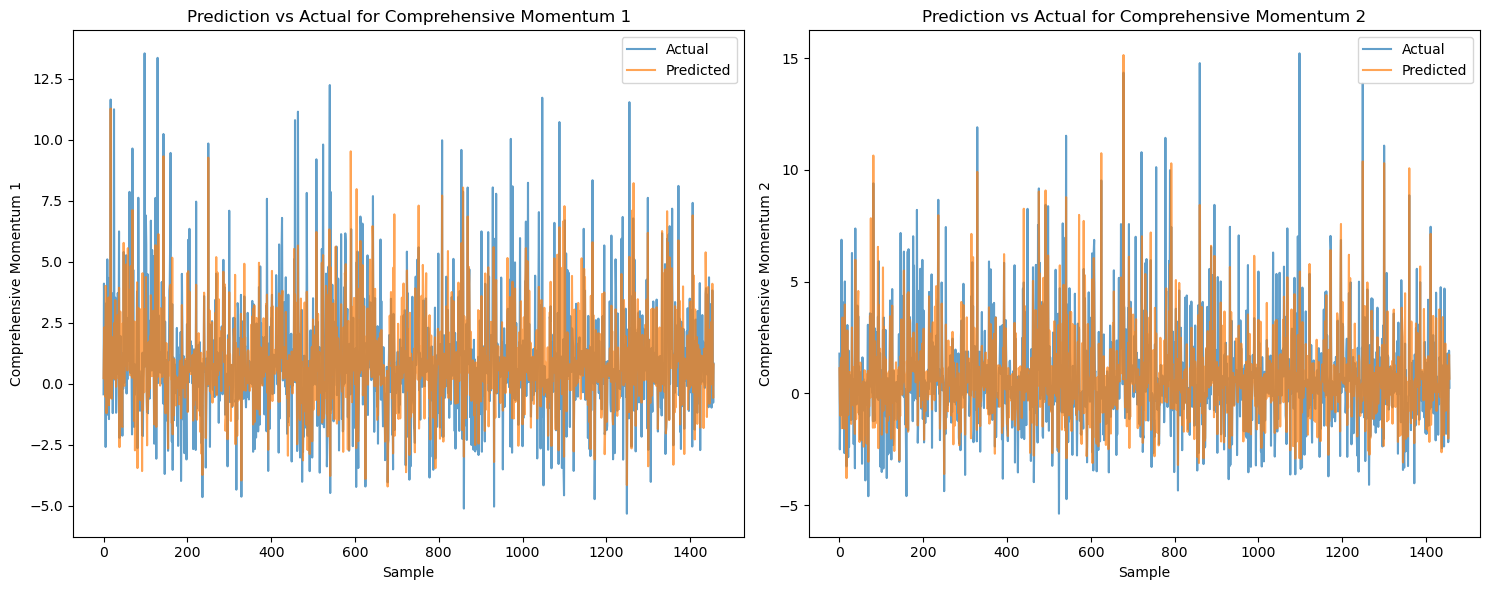
\includegraphics[width=.9\textwidth]{pred_act.png} %图片的名称或者路径之中有空格会出问题 
    \caption{Predicted curves vs Actual curves} % 图片标题 
    \label{pred_act}
\end{figure}

In the process of pinpointing crucial junctures and evaluating
the dynamics of the game, let's consider the match labeled as 1302.
The players involved in this encounter are Alexander Zverev, 
designated as Player 1 (P1), and Matteo Berrettini, 
referred to as Player 2 (P2).


\begin{table}[ht]
    \centering
    \resizebox{\textwidth}{!}{%
    \begin{tabularx}{\textwidth}{@{}c *{8}{X} c@{}}
    \toprule
    \makecell{Intersection} & \makecell{Game Point} & \makecell{Momentum\\1} & \makecell{Momentum\\2} & \makecell{Set} & \makecell{Game} & \makecell{Current\\Point} & \makecell{Result} & \makecell{Model\\Prediction} \\ \midrule
    1 & 26 & 0.65 & -0.71 & 0-0 & 1-2 & 40:15 (1st) & \makecell{Player 1 holds\\serve, 2-2} & \makecell{After this,\\Player 2\\has the upper\\hand} \\
    2 & 44 & -0.47 & 0.64 & 0-0 & 3-4 & 15:30 (1st) & \makecell{Player 2 scores,\\Player 1 error,\\15-40} & \makecell{Player 2\\further\\extends lead} \\
    3 & 64 & 0.36 & -0.44 & 0-1 & 1-1 & 40:0 (1st) & \makecell{Player 1 ace,\\2-1} & \makecell{Player 1\\turns the tide} \\
    4 & 112 & -0.81 & 0.82 & 0-1 & 6-6 & 15:40 (1st) & \makecell{Player 1 ace,\\30-40} & \makecell{Player 2\\retains advantage} \\
    5 & 135 & 2.16 & -3.30 & 0-2 & 1-1 & 30:40 (2nd) & \makecell{Player 2 holds\\serve, 1-2} & \makecell{Match\\reaches stalemate} \\ 
    \bottomrule
    \end{tabularx}
    }
    \caption{Tennis Match Detailed Analysis}
    \label{tab:tennis_analysis}
    \end{table}

\clearpage
\subsection{suggestion}
Although there is ambiguity in the increase or decrease of
momentum for individual points, considering the trend of 
the momentum curve and the actual events on the court, we 
believe our predictive model has successfully identified 
the key turning points that significantly affect the 
momentum of the match. Once these turning points are 
identified, we can extract them separately and analyze 
actual game strategies such as the types of serves and 
returns, the number of strokes, running distance, etc.

\begin{table}[ht]
\centering
\caption{Player1 as Server: Model Coefficients and Accuracy}
\begin{tabularx}{\textwidth}{@{}Xr@{}}
\toprule
Feature & Coefficient \\
\midrule
p1\_sets & -0.660716 \\
p2\_sets & 1.079027 \\
p1\_games & 0.523895 \\
p2\_games & -0.461889 \\
p1\_double\_fault & 0.360961 \\
p1\_unf\_err & -0.310627 \\
p2\_unf\_err & -0.924556 \\
rally\_count & 0.404886 \\
speed\_mph & -0.641765 \\
serve\_width\_B & -0.342782 \\
serve\_width\_BC & -0.237314 \\
serve\_width\_BW & -0.029538 \\
serve\_width\_C & 0.361789 \\
serve\_width\_W & 0.111184 \\
serve\_depth\_CTL & -0.393256 \\
serve\_depth\_NCTL & 0.391367 \\
distance\_diff & -0.314234 \\
p2\_distance\_run & -0.570710 \\
p1\_distance\_run & -0.515582 \\
\bottomrule
\end{tabularx}
\textbf{Model Accuracy:} 0.75
\end{table}

\begin{table}[ht]
\centering
\caption{Player1 as Receiver: Model Coefficients and Accuracy}
\begin{tabularx}{\textwidth}{@{}Xr@{}}
\toprule
Feature & Coefficient \\
\midrule
p1\_sets & 0.124868 \\
p2\_sets & -0.149697 \\
p1\_games & 0.519961 \\
p2\_games & -0.155793 \\
p2\_double\_fault & 0.643224 \\
p1\_unf\_err & -0.136075 \\
p2\_unf\_err & -0.087853 \\
rally\_count & -0.305280 \\
speed\_mph & 0.205257 \\
return\_depth\_D & 0.259512 \\
return\_depth\_ND & 0.372136 \\
distance\_diff & -0.093827 \\
p2\_distance\_run & 0.399639 \\
p1\_distance\_run & 0.333224 \\
\bottomrule
\end{tabularx}
\textbf{Model Accuracy:} 0.782608695652174
\end{table}

\subsection*{Recommendations for the Serving Player}
\begin{enumerate}
    \item Enhance First Serve Success: Increasing the success rate of first serves generally correlates with a stronger offensive position and reduced pressure.
    \item Diversify Serve Tactics: Utilizing a variety of serve trajectories (B, BC, BW, C, W) and depths (CTL, NCTL), servers are advised to dynamically alter their serving strategies to bewilder their opponents.
    \item Dictate Match Tempo: The rally\_count's positive impact implies that prolonging rallies may contribute to building momentum, likely linked to patient play, capitalizing on opponent errors, or generating scoring opportunities.
    \item Limit Unforced Errors: The significance of minimizing unforced errors, as indicated by the negative impact of p1\_unf\_err, highlights the need for consistency and error reduction.
\end{enumerate}

\subsection*{Guidance for the Receiving Player}
\begin{enumerate}
    \item Emphasize Defense and Counterplay: With their data reflecting the opponent's serve, receivers should prioritize defensive and responsive strategies.
    \item Strengthen Second Serve Returns: The coefficient related to p2\_double\_fault suggests an opportunity to increase aggression on second serve returns, targeting the opponent's weaknesses.
    \item Modify Return Techniques: Based on return\_depth\_D and return\_depth\_ND, receivers should adapt their positioning and return tactics in response to ongoing match conditions.
    \item Optimize Movement Efficiency: By effectively managing movement on the court, receivers can reduce unnecessary exertion, preserving energy and focus.
\end{enumerate}
\section{Model generalization detection}
















\section{Conclusion}
In the final analysis of this report, it must be acknowledged that due to the experimental team's inability to complete the experimental tasks in a timely manner, the objectives set for the third part of the study were not realized. Consequently, we are only able to provide the predictive outcomes for sea water temperature and fish migration patterns in the Scottish region. The analysis and conclusions regarding these two outcomes have already been discussed in their respective sections, and thus will not be reiterated here. Regrettably, from the perspective of serving as consultants for Scottish fishing companies, this experiment was unequivocally a failure. We must concede that this report fails to offer any valuable insights or recommendations for the strategic operations of fishing companies.


% 参考文献,此处以 MLA 引用格式为例
\clearpage   %另起一页继续写。这时,你最好使用“\clearpage” 
\begin{thebibliography}{99}
	\bibitem{1} HU Teng, LIU Zhanjun, LIU Yang, et al. 3D reconnaissance path planning of multiple UAVs. Journal of Systems Engineering and Electronics, 2019, 41(7): 1551-1559.
	\bibitem{2} BASBOUS B. 2D UAV path planning with radar threatening areas using simulated an-nealing algorithm for event detection. The 2018 International Conference on Artificial Intelligence and Data Processing. Malatya, Turkey: IEEE,2018: 1-7.
	\bibitem{3} WANG W F, WU Y C, ZHANG X. Research of the unit decomposing traversal method based on grid method of the mobile robot. Techniques of Automation and Applications, 2013, 32(11): 34-38.
	\bibitem{4} XU Jian, ZHOU Deyun, HUANG He. Multi UAV path planning based on improved ge-netic algorithm. Aeronautical Computing Technique, 2009, 39(4): 43-46.

\end{thebibliography}
% \includepdf[pages={1,2}]{Memo.pdf} 

\end{document}  % 结束